%%%%%%%%%%%%%%%%%%%%%%%%%%%%%%%%%%%%%%%%%%%%%%%%%%%%%%%%%%%%%%%%%%%%%%%%

\documentclass{beamer}
\mode<presentation> {
\usetheme{Madrid}
\setbeamercovered{invisible}
\setbeamertemplate{navigation symbols}{} 
}


\usepackage[italian]{babel}
\usepackage{graphicx}
\usepackage{amssymb}
\usepackage[T1]{fontenc}
%\usepackage{bm} 
\logo{
\includegraphics[height=1.2cm]{unipd.png}}
\title[Data Mining]{Analisi di un Servizio di Bike Sharing}
\author{Marco Zanella}
\institute[Universit\`a di Padova]
{
Universit\`a di Padova \\
\medskip
{\emph{marco.zanella.9@studenti.unipd.it}}
}
\date{\today}



\begin{document}
\begin{frame}
\titlepage
\end{frame}


\begin{frame}{Table of Contents}
\tableofcontents
\end{frame}



\section{Motivazione}
\begin{frame}{Motivazione}

I servizi di bike-sharing generano enormi quantit\`a di dati:
ottimi per tecniche di \emph{data-mining}.

\begin{center}
  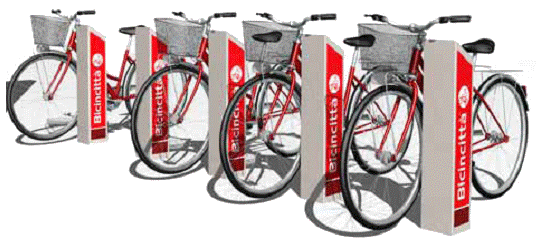
\includegraphics[height=0.3\textheight]{images/bike-sharing.png}
\end{center}

Predire la quantit\`a di utenti: migliore organizzazione
delle rastrelliere e degli interventi di manutenzione.

\begin{thebibliography}{99}
  \bibitem[Label1, 2013]{key1} Hadi Fanaee-T and Joao Gama
  \newblock Event labeling combining ensemble detectors and background knowledge
\end{thebibliography}
\end{frame}



\section{Analisi preliminare}
\subsection{Significato delle variabili}
\begin{frame}{Analisi preliminare - I predittori}
I predittori sono fattori esterni e/o ambientali:
\begin{itemize}
  \item temperatura
  \item orario
  \item giorno festivo/feriale
  \item ...
\end{itemize}

Possono avere importanza diversa, essere ridondanti o erronei:
\begin{center}
  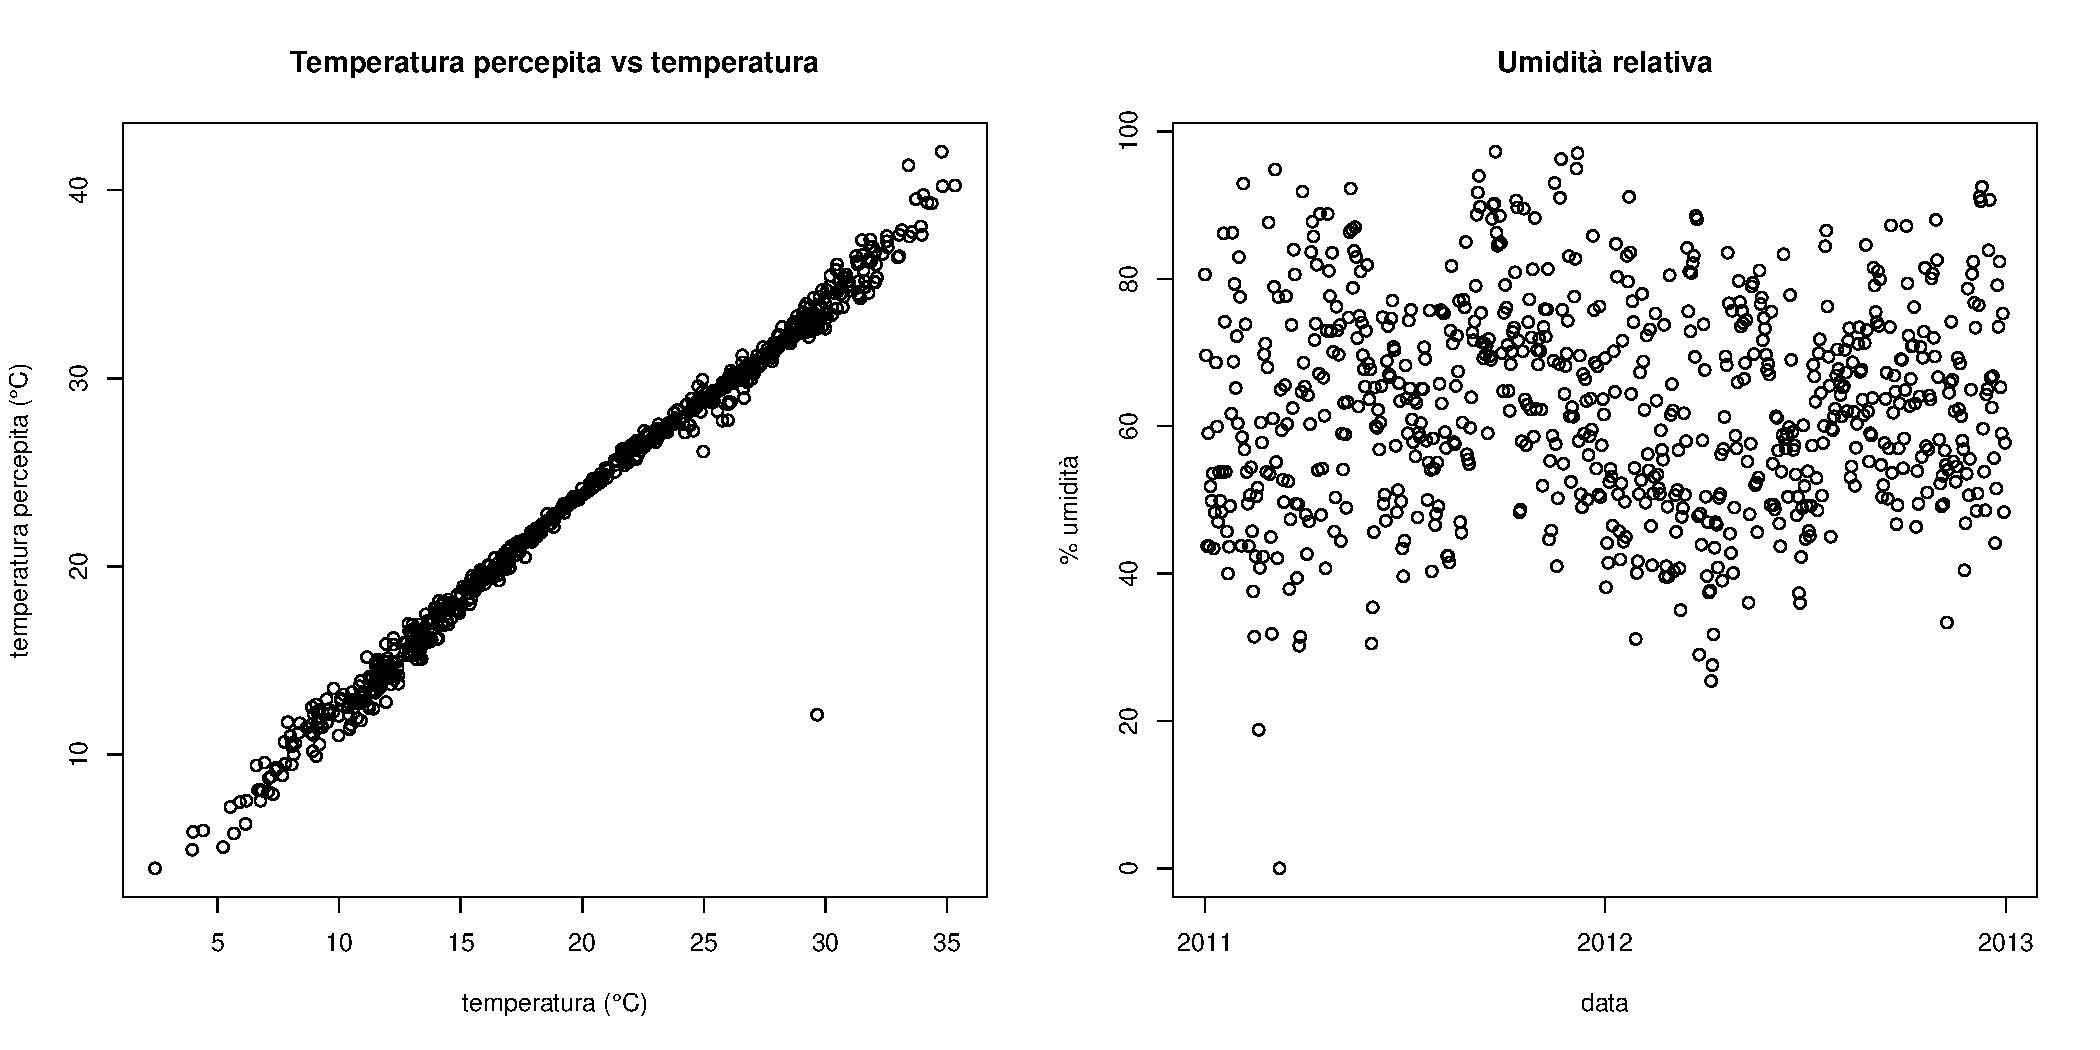
\includegraphics[height=0.3\textheight]{images/temperature-humidity.pdf}
\end{center}
Nel dataset, non ci sono informazioni mancanti.
\end{frame}


\begin{frame}{Analisi preliminare - I predittori}
\`E possibile raggruppare alcune informazioni, come le ore:
\begin{center}
  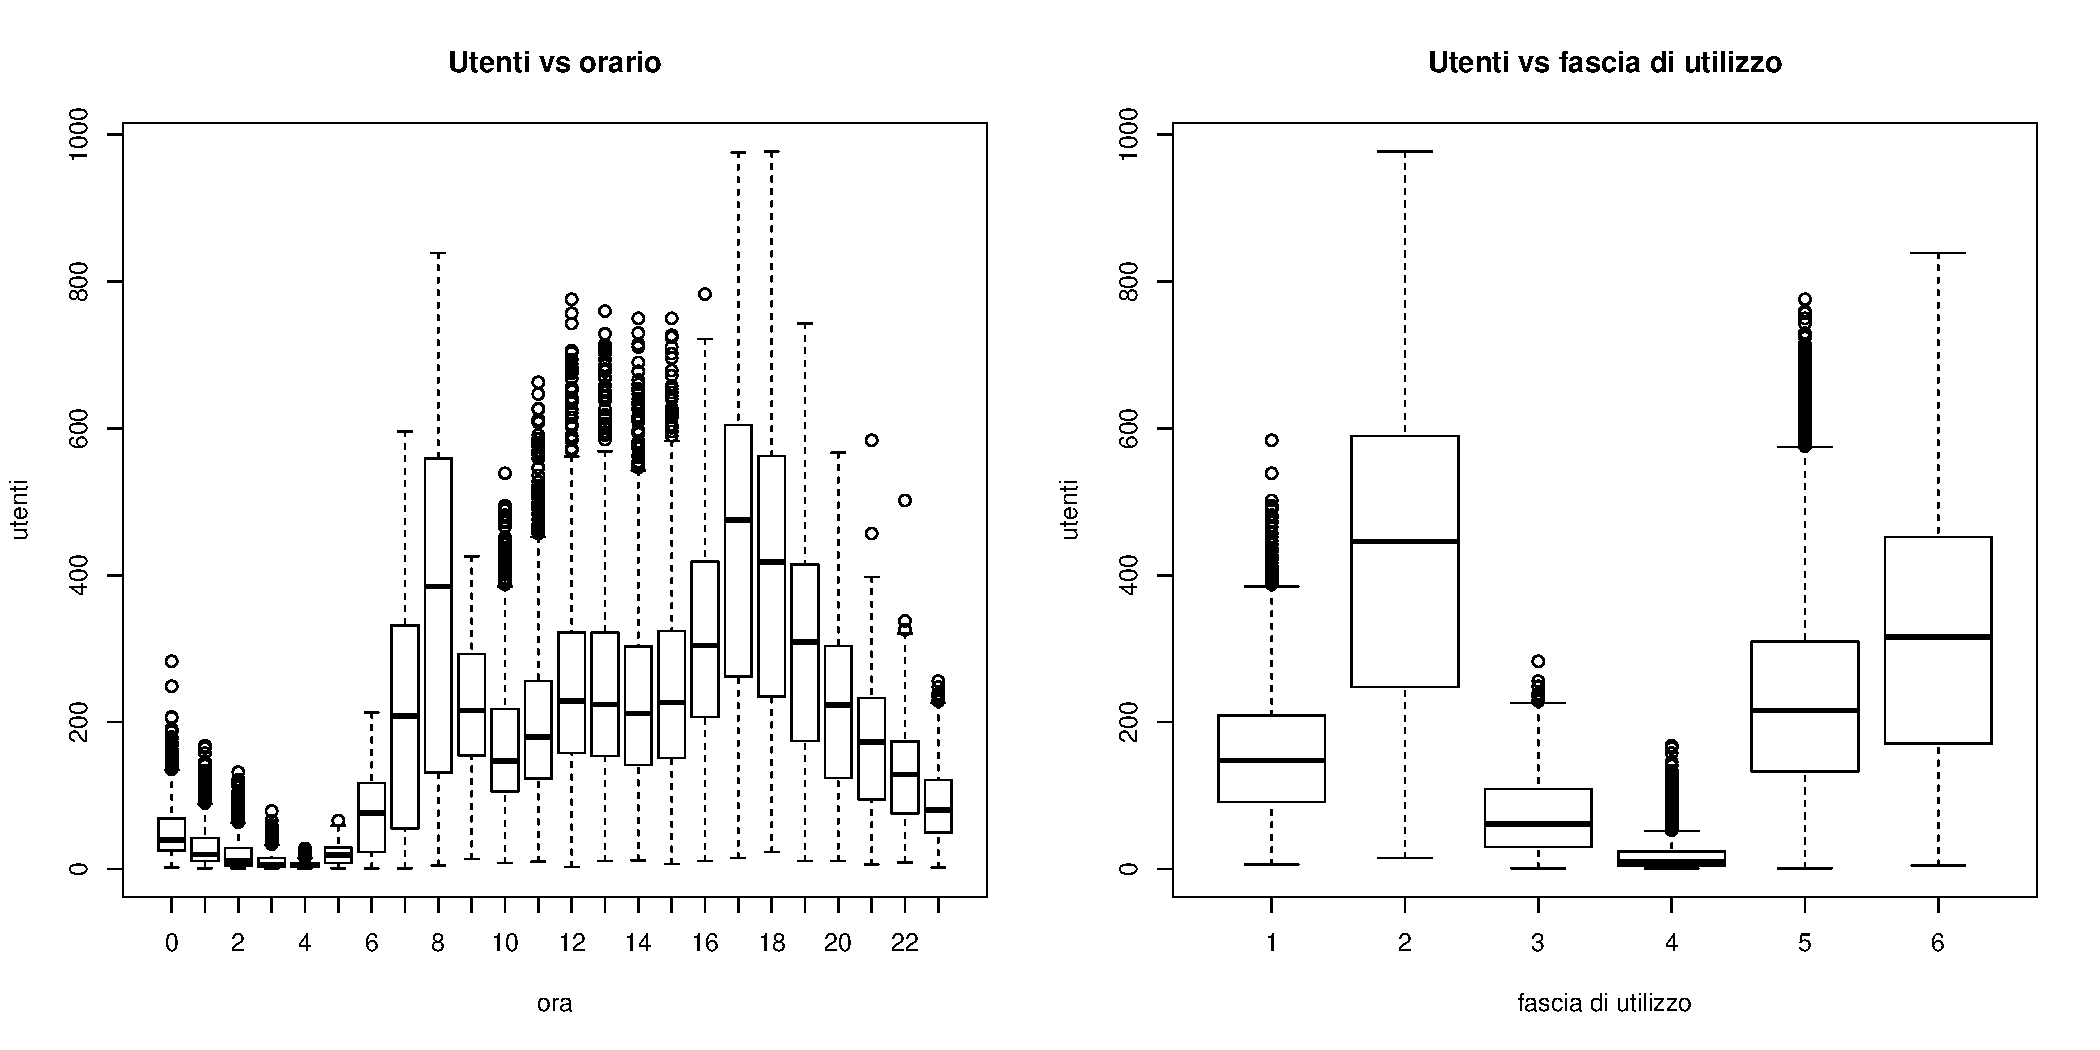
\includegraphics[height=0.5\textheight]{images/hour-timeslot.pdf}
\end{center}
Gli algoritmi di \emph{clustering} automatizzano il processo.
\end{frame}




\subsection{Individuazione degli outlier}
\begin{frame}{Analisi preliminare - Outlier}
Punti "sospetti", apparentemente anomali.
\begin{center}
  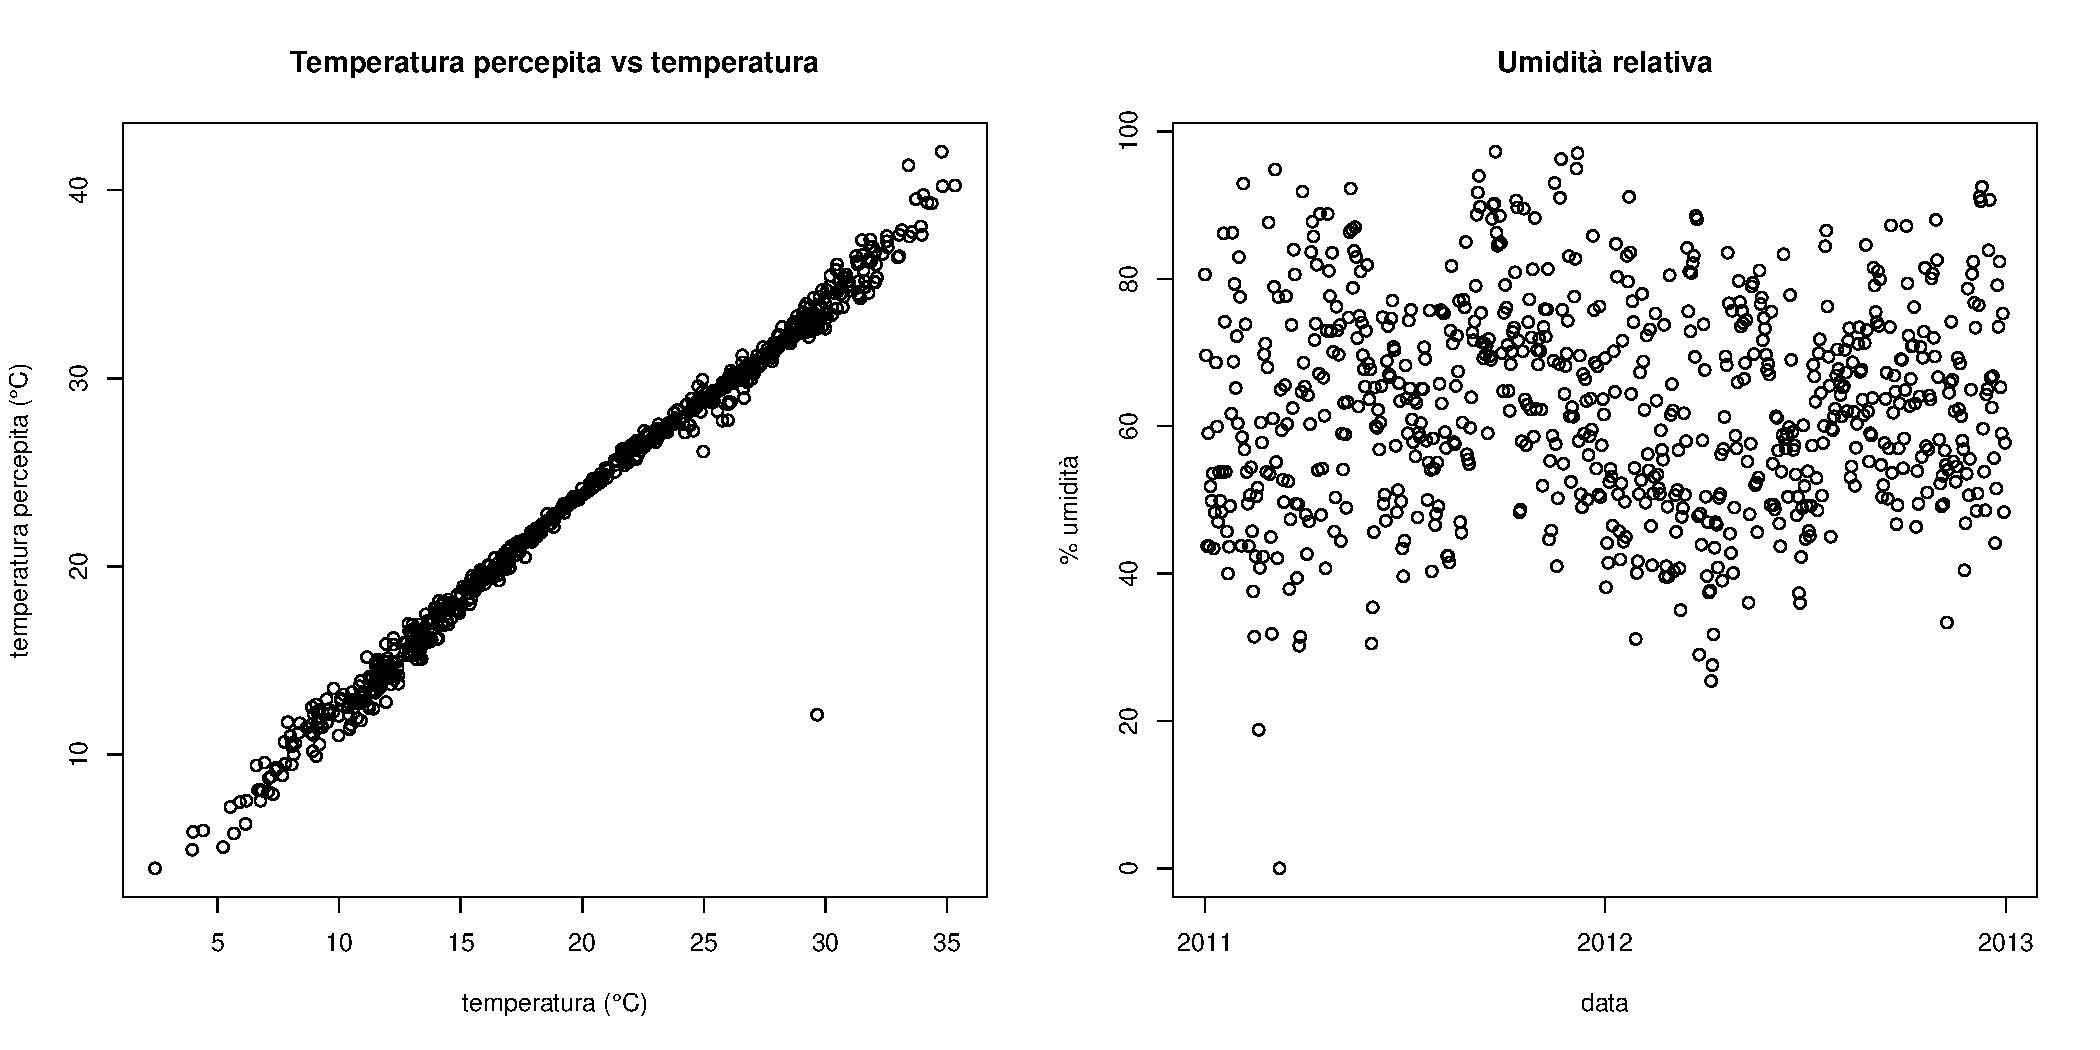
\includegraphics[height=0.5\textheight]{images/temperature-humidity.pdf}
\end{center}
Richiedono un'investigazione manuale per valutarne mantenimento o rimozione.
\end{frame}



\section{Regressione}
\subsection{Modelli utilizzati}
\begin{frame}{Regressione - I modelli}
I modelli sono costruiti su un \emph{insieme di stima} (75\% delle osservazioni):
\begin{itemize}
  \item modello lineare
  \item MARS (con 1 e 2 gradi di interazione)
  \item GAM (con loess e splines)
  \item Projection Pursuit Regression
  \item Rete neurale
  \item Albero CART
\end{itemize}
Eventuali parametri sono stimati attraverso una scansione, suddividendo
l'insieme di stima in \emph{insieme di costruzione} e \emph{di controllo}.
\end{frame}

\subsection{Confronto dei risultati}
\begin{frame}{Regressione - Risultati}
I risultati sono valutati in termini di MSE (\emph{Mean Squared Error},
errore quadratico medio) sull'\emph{insieme di verifica}.

\begin{table}
  \centering
  \begin{tabular}{|| l | r | r ||}
    \hline
    modello       & variabili       & MSE      \\
    \hline \hline
    Lineare       & tutte           & 12664.50 \\
    Lineare       & solo sign.      & 13056.61 \\
    MARS          & tutte (grado 1) & 12619.53 \\
    MARS          & tutte (grado 2) &  6596.50 \\
    GAM (splines) & tutte           & 12643.32 \\
    GAM (splines) & solo sign.      & 12998.99 \\
    GAM (loess)   & tutte           & 12602.14 \\
    GAM (loess)   & solo sign.      & 12975.89 \\
    PPR           & 6 termini       &  5206.72 \\
    Rete neurale  & -               &  9172.46 \\
    CART          & 50  foglie      &  7347.62 \\
    CART          & 13  foglie      & 10449.94 \\
    \hline
  \end{tabular}
\end{table}
\end{frame}



\section{Classificazione}
\begin{frame}{Classificazione}
Quanti utenti sono occasionali? In quali circostanze sono pi\`u attivi?

\begin{center}
  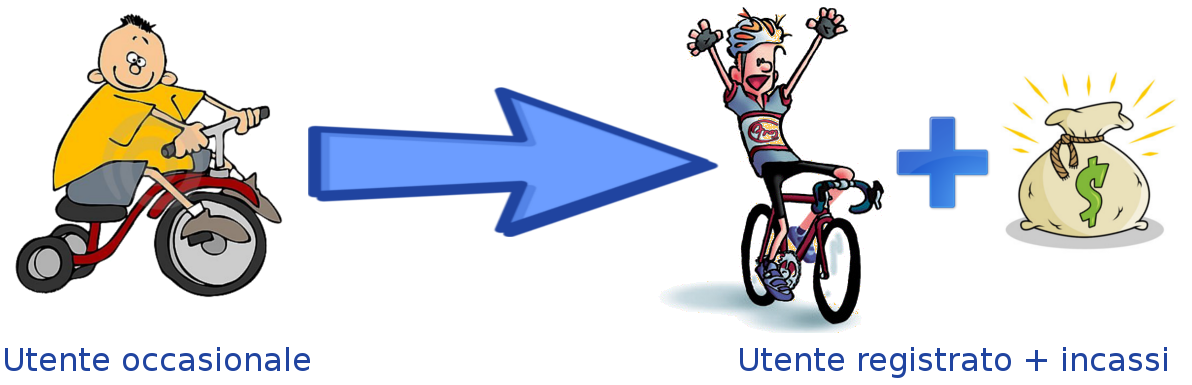
\includegraphics[width=0.9\textwidth]{images/conversion.png}
\end{center}


Gli utenti registrati portano guadagni maggiori: identificare gli utenti
occasionali e convertirli in registrati.
\end{frame}


\subsection{Modelli utilizzati}
\begin{frame}{Classificazione - I modelli}
Modelli allenati sull'\emph{insieme di stima}:
\begin{itemize}
  \item modello lineare
  \item CART (classificazione)
  \item CART (regressione)
  \item MARS
  \item bagging
  \item boosting
  \item random forest
\end{itemize}
I modelli che producono valori \emph{quantitativi} usano delle \emph{soglie}
per ottenere le \emph{classi}.
\end{frame}

\subsection{Confronto dei risultati}
\begin{frame}{Classificazione - Risultati}
L'errore totale di classificazione viene usato come metrica.
\begin{table}
  \centering
  \begin{tabular}{|| l | r ||}
    \hline
    Modello                & errore \\
    \hline
    lineare                & 0.34   \\
    CART - classificazione & 0.31   \\
    CART - regressione     & 0.31   \\
    MARS                   & 0.34   \\
    bagging                & 0.29   \\
    boosting               & 0.28   \\
    random forest          & 0.26   \\
    \hline
  \end{tabular}
\end{table}
\end{frame}


\begin{frame}{Classificazione - Risultati}
Gli errori sono molto simili: curve lift e ROC possono aiutare.
\begin{center}
  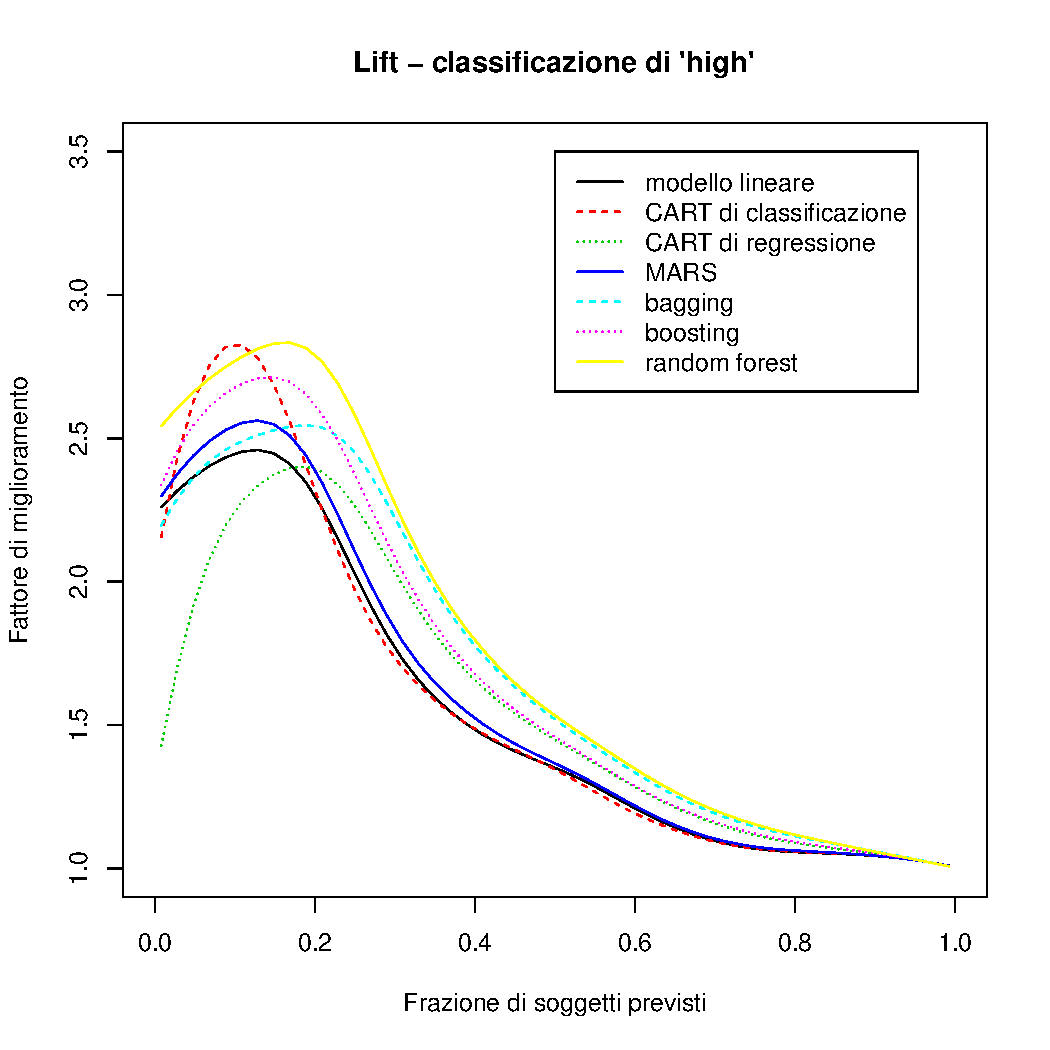
\includegraphics[width=0.45\textwidth]{images/lift-high.pdf}
  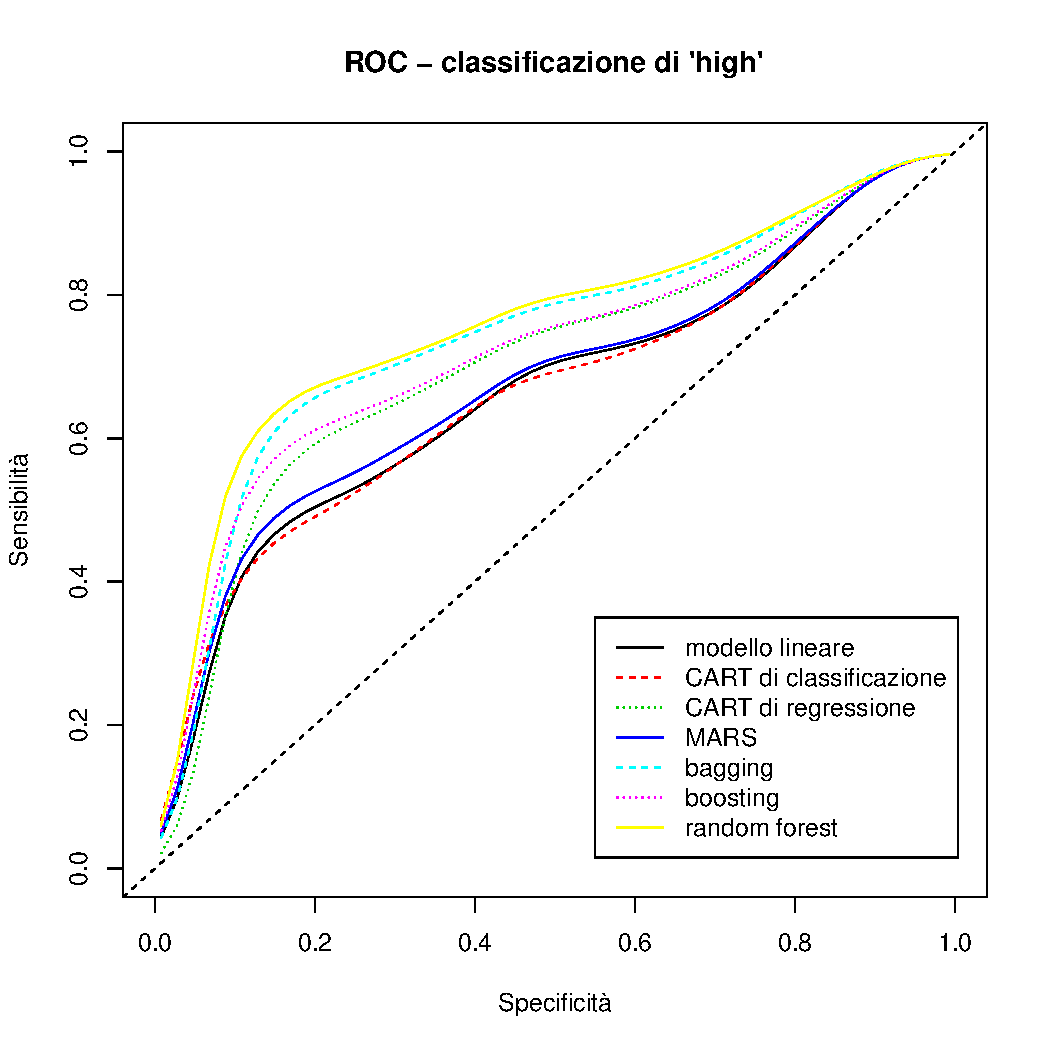
\includegraphics[width=0.45\textwidth]{images/roc-high.pdf}
\end{center}
Il nostro interesse \`e maggiormente verso la
classe \emph{high}.
\end{frame}



\begin{frame}{Classificazione - Risultati}
Una piccola verifica informale: predire il numero di utenti casuali
con i risultati ottenuti.

\begin{center}
  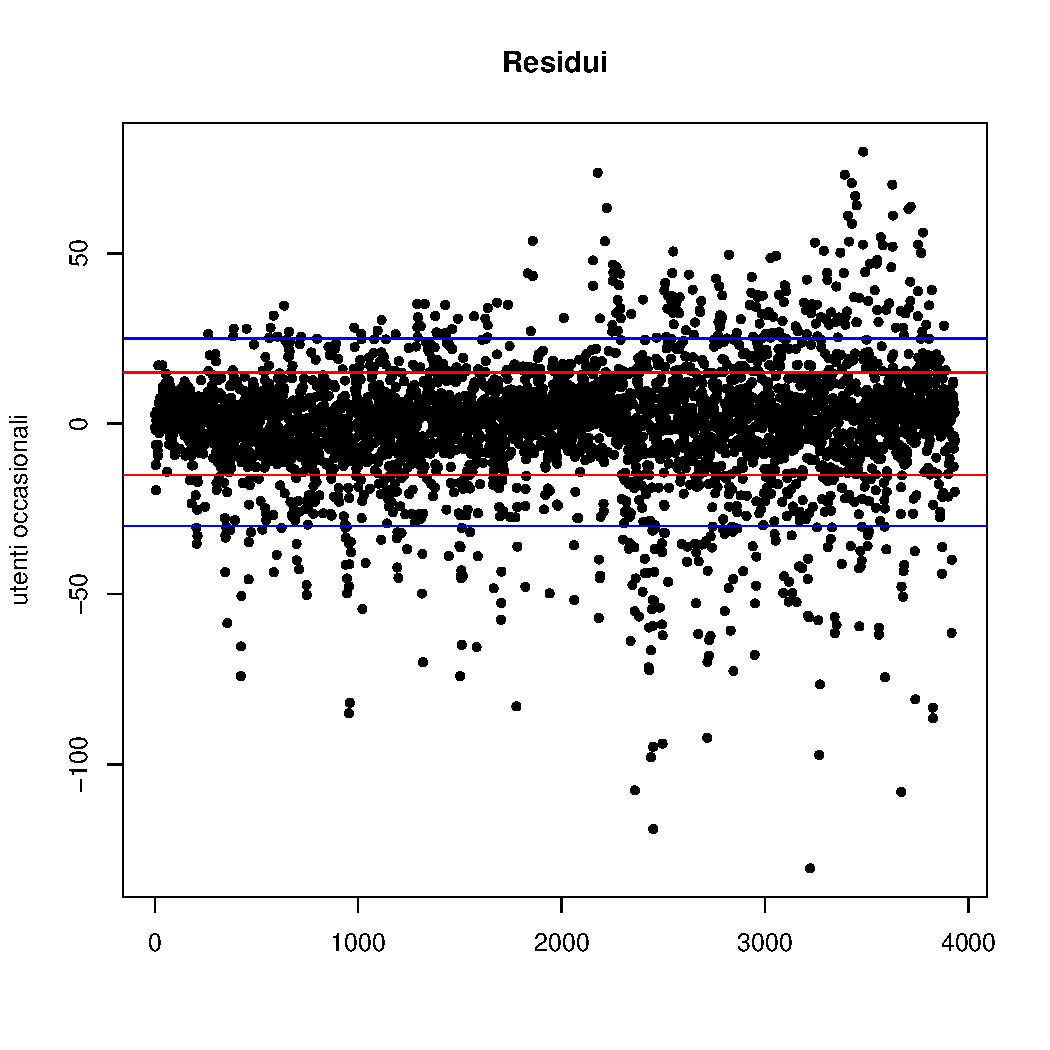
\includegraphics[height=0.5\textheight]{images/classification-residuals.pdf}
\end{center}

Residui \emph{ben distribuiti}, $R^{2} = 0.89$.
\end{frame}







\begin{frame}{Conclusione -- Grazie!}
\begin{block}{Conclusione - Regressione}
\begin{itemize}
  \item Analisi preliminare approfondita
  \item Diversi modelli esaminati e confrontati
  \item Scansioni esaustive per la stima dei parametri {\tiny (regressione)}
  \item Buoni risultati in termini di \emph{MSE} {\tiny (regressione)}
  \item Buoni risultati in termini di errore, ROC e lift {\tiny (classificazione)}
  \item Verifica informale del classificatore positiva
\end{itemize}
\end{block}

\begin{block}{Domande?}
\end{block}
\end{frame}


\end{document}